\section{Framework}
\label{sec:framework}

We present \texttt{nl2atl}, the open-source framework that operationalizes the translation of natural-language strategic requirements into well-formed ATL/ATL$^\ast$ specifications. Its design comprises three components: a \emph{hybrid inference} layer that runs local open-weight models and cloud APIs behind a single interface; \emph{scalable and reproducible} experimentation with multi-seed aggregation and cluster execution; and \emph{post-prediction evaluation} that couples syntactic and meaning-level assessment and feeds directly into a strategic model checker. Figure~\ref{fig:tool_pipeline} sketches the architecture; the end-to-end translation-and-evaluation loop is given as Algorithm~1 in the technical appendix.

\usetikzlibrary{arrows.meta, positioning, fit, backgrounds, calc}
\begin{figure}[t]
\centering
\resizebox{0.9\columnwidth}{!}{%
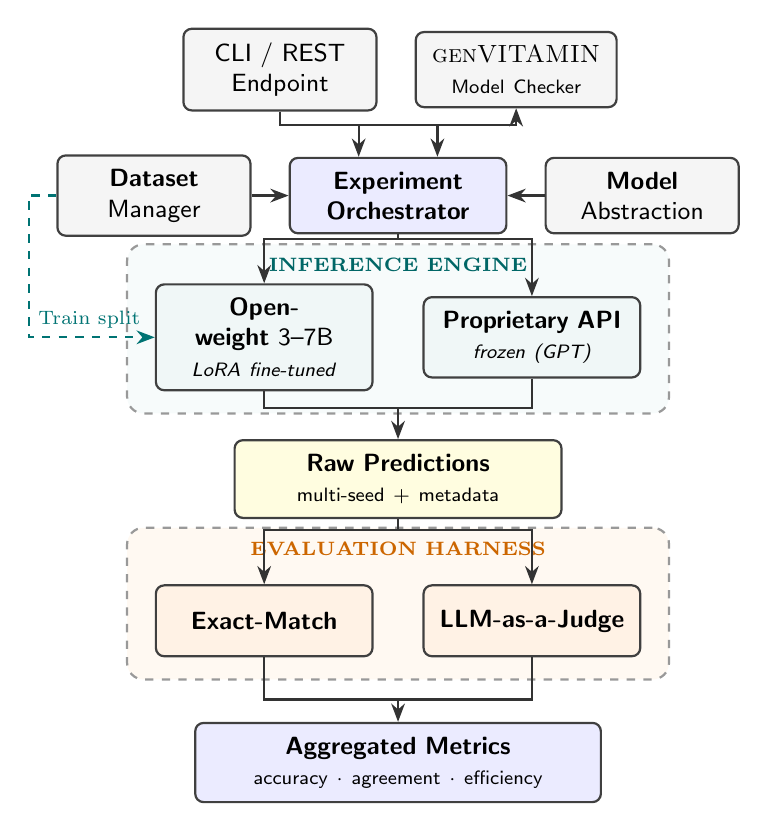
\begin{tikzpicture}[
    font=\small\sffamily,
    >=Stealth,
    % Standard box styles
    box/.style={
        rectangle, draw=black!75, thick, rounded corners=3pt,
        align=center, fill=white, minimum height=9mm, inner sep=5pt
    },
    io/.style={box, fill=gray!8},
    core/.style={box, fill=blue!8},
    data/.style={box, fill=yellow!12},
    infer/.style={box, fill=teal!6},
    eval/.style={box, fill=orange!10},
    % Grouping box styles
    grp/.style={
        rectangle, draw=black!40, thick, dashed, rounded corners=6pt,
        inner xsep=10pt, inner ysep=8pt
    },
    % Arrow styles
    arr/.style={->, thick, draw=black!80},
    trainarr/.style={->, thick, dashed, draw=teal!90!black},
    line/.style={thick, draw=black!80}
]

% ==========================================
% NODES & PLACEMENT
% ==========================================

% --- Core Architecture (Level 1) ---
\node[core, text width=2.4cm] (orch) at (0, 3) {\textbf{Experiment}\\\textbf{Orchestrator}};
\node[io, text width=2.1cm] (dm) at (-3.1, 3) {\textbf{Dataset}\\Manager};
\node[io, text width=2.1cm] (mal) at (3.1, 3) {\textbf{Model}\\Abstraction};

% --- Inputs (Level 0) ---
% Positioned slightly inward to ensure downward lines cleanly avoid the DM/MAL boxes
\node[io, text width=2.1cm] (cli) at (-1.5, 4.6) {CLI / REST\\Endpoint};
\node[io, text width=2.2cm] (vit) at (1.5, 4.6) {\textsc{genVITAMIN}\\{\scriptsize Model Checker}};

% --- Inference Engine (Level 2) ---
\node[infer, text width=2.4cm] (local) at (-1.7, 1.2) {\textbf{Open-weight} 3--7B\\{\scriptsize \textit{LoRA fine-tuned}}};
\node[infer, text width=2.4cm] (cloud) at (1.7, 1.2) {\textbf{Proprietary API}\\{\scriptsize \textit{frozen (GPT)}}};

% --- Raw Predictions (Level 3) ---
\node[data, text width=3.8cm] (pred) at (0, -0.6) {\textbf{Raw Predictions}\\{\scriptsize multi-seed $+$ metadata}};

% --- Evaluation Harness (Level 4) ---
\node[eval, text width=2.4cm] (em) at (-1.7, -2.4) {\textbf{Exact-Match}};
\node[eval, text width=2.4cm] (judge) at (1.7, -2.4) {\textbf{LLM-as-a-Judge}};

% --- Final Output (Level 5) ---
\node[core, text width=4.8cm] (metrics) at (0, -4.2) {\textbf{Aggregated Metrics}\\{\scriptsize accuracy $\cdot$ agreement $\cdot$ efficiency}};

% ==========================================
% BACKGROUND GROUPINGS
% ==========================================
\begin{scope}[on background layer]
    % Inference Engine Group
    \coordinate (inf_top) at (0, 2.1);
    \node[grp, fill=teal!3, fit=(local)(cloud)(inf_top)] (inf_box) {};
    \node[below=2pt of inf_box.north, font=\bfseries\scriptsize\color{teal!80!black}] {INFERENCE ENGINE};

    % Evaluation Harness Group
    \coordinate (eval_top) at (0, -1.5);
    \node[grp, fill=orange!5, fit=(em)(judge)(eval_top)] (eval_box) {};
    \node[below=2pt of eval_box.north, font=\bfseries\scriptsize\color{orange!80!black}] {EVALUATION HARNESS};
\end{scope}

% ==========================================
% ROUTING & ARROWS
% ==========================================

% 1. Inputs to Orchestrator
\draw[arr] (cli.south) |- (0, 3.9) -| ([xshift=-0.5cm]orch.north);
\draw[<->, thick, draw=black!80] (vit.south) |- (0, 3.9) -| ([xshift=0.5cm]orch.north);

% 2. DM and MAL to Orchestrator
\draw[arr] (dm.east) -- (orch.west);
\draw[arr] (mal.west) -- (orch.east);

% 3. DM to Local Model (Train Split fine-tuning loop)
% Wraps cleanly around the outside left edge
\draw[trainarr] (dm.west) -- ++(-0.35, 0) |- (local.west) 
    node[pos=0.74, above, font=\scriptsize\color{teal!90!black}, inner sep=3pt] {Train split};

% 4. Orchestrator fork to Inference
\draw[line] (orch.south) -- (0, 2.45);
\draw[arr] (0, 2.45) -| (local.north);
\draw[arr] (0, 2.45) -| (cloud.north);

% 5. Inference merge to Predictions
\draw[line] (local.south) |- (0, 0.3);
\draw[line] (cloud.south) |- (0, 0.3);
\draw[arr] (0, 0.3) -- (pred.north);

% 6. Predictions fork to Evaluators
\draw[line] (pred.south) -- (0, -1.25);
\draw[arr] (0, -1.25) -| (em.north);
\draw[arr] (0, -1.25) -| (judge.north);

% 7. Evaluators merge to Metrics
\draw[line] (em.south) |- (0, -3.4);
\draw[line] (judge.south) |- (0, -3.4);
\draw[arr] (0, -3.4) -- (metrics.north);

\end{tikzpicture}%
}
\caption{The \texttt{nl2atl} architecture. A natural-language requirement (from the CLI, a REST endpoint, or the integrated \textsc{genVITAMIN} model checker) reaches the \emph{Experiment Orchestrator}, which draws stratified splits and exemplars from the \emph{Dataset Manager} and resolves models through the \emph{Model Abstraction Layer}. Inference is hybrid: open-weight $3$--$7$B models are LoRA fine-tuned and served locally (dashed arrow), while proprietary API models are used frozen, behind one interface. Each generation is stored as a multi-seed raw prediction and scored by two independent evaluators (exact match and an LLM-as-a-judge) before aggregation into accuracy, agreement, and efficiency metrics.}
\label{fig:tool_pipeline}
\end{figure}

\subsection{Architecture}
Requests enter through a command-line interface or a REST endpoint and reach an \textbf{Experiment Orchestrator}. It draws data from a \textbf{Dataset Manager} (which produces deterministic, stratified train/validation/test partitions and holds the curated few-shot exemplars out of every split, so no prompting example leaks into evaluation) and resolves models through a \textbf{Model Abstraction Layer}, a declarative registry mapping a short model key to its provider, checkpoint, decoding parameters, and fine-tuning targets. The backing \textbf{Inference Engine} serves local open-weight checkpoints and cloud endpoints under one calling convention; because fine-tuning depends on initialization, each fine-tuned configuration is repeated over several seeds, while greedy decoding keeps run-to-run variation attributable to training rather than sampling. Every generation is stored as a \emph{raw prediction} with its metadata (latency, token counts, decoding configuration) before any scoring, and two evaluators then consume it: an \textbf{Exact-Match Evaluator} for normalized syntactic comparison and an \textbf{LLM-as-a-Judge} for meaning when surface forms diverge. Decoupling inference from evaluation, and applying the same two-tier scoring to local and cloud predictions alike, ensures that observed differences reflect model capability rather than the harness.

\subsection{Prompting and Output Parsing}
\label{subsec:prompting}
The translation target is pinned by a system prompt that fixes the ATL/ATL$^\ast$ surface syntax (the coalition modality $\langle\!\langle A \rangle\!\rangle$, the temporal operators $X$, $F$, $G$, and $U$, the Boolean connectives, \textsc{PascalCase} agent names, and \texttt{snake\_case} atomic propositions) together with the scope convention that keeps the strategic operator separate from the temporal operator it governs, e.g.\ $\langle\!\langle \mathrm{Machine}\rangle\!\rangle\,G(\mathit{paid}\rightarrow \mathit{printed})$ rather than $\langle\!\langle \mathrm{Machine}\rangle\!\rangle(G\,\mathit{paid}\rightarrow \mathit{printed})$. It also states the intended treatment of each targeted ambiguity: repeat the recovered formula for VP ellipsis, share the right-peripheral objective across both conjuncts for Right Node Raising, and emit \emph{all} admissible readings (one per line) for quantifier-scope ambiguity, never fusing two distinct readings into one. The few-shot condition prepends a small curated pool of exemplars spanning these phenomena, held out of every split. Models emit plain text under greedy decoding; a parser then strips extraneous tokens and canonicalizes whitespace, letter case, and operator spelling, so that scoring compares formulas rather than incidental surface form. A requirement with several readings is stored as a set of gold formulas, and a prediction must reproduce the entire set to count as correct. The full system prompt and the curated few-shot exemplars are reproduced in the technical appendix.

\subsection{Hybrid Inference: Privacy and Capacity}
\label{subsec:hybrid}
Confidentiality of requirements is a central concern in industrial formal methods, so the framework treats local open-weight inference as a primary path: checkpoints are fine-tuned with low-rank adapters~\cite{hu2022lora}, with $4$-bit QLoRA quantization~\cite{dettmers2023qlora} for the larger $7$B models, enabling domain specialization entirely on-premises, with no requirement leaving the air-gapped environment. The same interface targets Azure OpenAI endpoints when data sensitivity permits, letting practitioners trade data sovereignty against reasoning capacity without altering the pipeline.

\subsection{Scalability and Reproducibility}
\label{subsec:scale}
The framework targets large parameter sweeps over models, prompting conditions, and seeds: each $(\text{model}, \text{condition}, \text{split})$ cell is an independent unit of work dispatched to a SLURM-managed GPU cluster. To separate genuine capability from initialization noise, the orchestrator \emph{decouples} the data-split seed from the training seed and supports two protocols: a single \emph{canonical} stratified split, identical across models, used for the headline numbers reported here, and an optional stratified $k$-fold cross-validation mode, with shared folds, for estimating split-induced variance. Aggregation runs on the appropriate axis (over seeds or folds), yielding means with dispersion rather than single-point estimates.

\subsection{Model-Checker Integration}
\label{subsec:integration}
The practical value of a translation depends on its usability inside a verification workflow. We therefore connect \texttt{nl2atl} to \textsc{genVITAMIN}, an established model checker for strategic logics~\cite{DBLP:conf/ifaamas/0001M25}, so designers can express constraints in natural language and obtain formulas that are immediately parsed and verified (a screenshot is provided in the technical appendix). The integration is decoupled and dual-service: the verification backend manages the model-checking environment, while translation runs as a FastAPI microservice exposing a \texttt{/generate} endpoint that takes the requirement, a model key, and prompting flags (few-shot, maximum new tokens, and an optional fine-tuned adapter). A non-destructive patch installs a thin client so that ATL requests are routed to the translation service first and transparently fall back to the checker's native generation whenever the service is unavailable or returns an ill-formed result. Because the emitted formulas are parsed by the same front-end used for verification, only well-formed specifications enter model checking, giving immediate syntactic validation of model output.